%https://www.overleaf.com/learn/latex/Creating_a_document_in_LaTeX
\documentclass[13pt]{report}
\usepackage{graphicx}
\usepackage{listings}

\title{CS 440: Inference-Informed Action}
\author{Steven Nguyen \& Kyra Kennedy}
\date{19 March 2021}

\begin{document}

\begin{titlepage}
\maketitle
\end{titlepage}

\section*{Abstract}
In this project, we demonstrate how to collect data and infer information for future actions using agents that play minesweeper.

\section*{Academic Integrity}
It was agreed from when we first started that Steven Nguyen would handle the Basic Agent and the board representation while Kyra Kennedy worked on the Improved Agent. Both members assisted in this write up.\\
I, Steven Nguyen, have not copied our code or taken from online or another student's work.\\
I, Kyra Kennedy, have not copied our code or taken from online or another student's work.

\break
\section*{Basic Agent}
The basic agent is a simple agent for handling minesweeper. This assumes a hidden tile is safe only when a all the bombs around a visible tile are already visible. This assumes a hidden tile is a bomb only when the number of hidden tiles around a tile matches the clue on a tile.

\subsection*{Representation}
The board was represented with a Numpy 2darray in which bombs are represented by 1s and safe tiles are represented with 0s. The basic agent used a dictionary of cells indexed by board positions to store the knowledge base. In a cell's information, we stored: if the cell is a bomb, a list of the positions of all of its neighbors, a list of the positions of the neighbors that are revealed to be not bombs, a list of the positions of the neighbors that are revealed to be bombs, a list of the positions of unrevealed neighbors, and the integer clue if the cell has been queried.When a relationship between 2 cells is updated, the relevant lists of relationships in both cells are updated.

\subsection*{Inference}
When a new cell is queried, if it is a bomb, we first mark the cell as a bomb and update all of its relationships to display it as a bomb and to display it as not hidden anymore. If the queried cell is not a bomb, then we use the clue to determine if the surrounding hidden cells are either all bombs or all not bombs. For each hidden cells that gets updated, we repeat this process. Then, in each visible neighbor, we check if the surrounding hidden cells are either all bombs or all not bombs in case revealing a cell has allowed us to declare hidden cells as all bombs or all not bombs. For each hidden cells that gets updated, we repeat this process.\\
Assuming the strongest inference this agent can make is if a queried cell's surrounding hidden tiles are all bombs or all not bombs, yes, this is all we can deduct from a given clue. This is because when a cell is changed, only its direct neighbors can be affected, so, since this agent is checking all of the direct neighbors for new inferences, everything deductable is detected.

\subsection*{Decisions}
Given that there are no queried tiles or no tiles with clues, all tiles have the same probability of being queried randomly. After a tile is queried, and its neighbors are checked to be all bombs or all not bombs, all of it's visible neighbors will be checked in case their surrounding tiles are all bombs or all not bombs. After any tile is marked to be a bomb or safe from checking if another tile is surrounded by all bombs or not all bombs, the tile will be queried if not a bomb and then all of it's neighbors will be checked to be all bombs or all not bombs. Given that there is at least 1 tile marked as a bomb or 1 tile marked as safe, all hidden tiles will have the same probability of being queried randomly to do the same process as above.

\subsection*{Decision Performance}
\begin{verbatim}
>>> import board           
>>> import basic_agent
>>> b = board.Board(6, 8)
>>> agent = basic_agent.Agent(b) 
>>> agent.run()
Running basic agent with a 6x6 board
Querying (3, 5)
Hit a bomb
Querying (4, 5)
Received clue: 1
Marking (4, 5) as safe and as visible to all neighbors
Checking hidden neighbors of (4, 5)
All hidden neighbors are safe
Marking (5, 5) as safe and as visible to all neighbors
Marking (5, 4) as safe and as visible to all neighbors
Marking (4, 4) as safe and as visible to all neighbors
Marking (3, 4) as safe and as visible to all neighbors
Scanning neighbors of (4, 5) that are deemed safe
Querying (5, 5)
Received clue: 0
Marking (5, 5) as safe and as visible to all neighbors
Checking hidden neighbors of (5, 5)
Nothing has been found in hidden neighbors
Scanning neighbors of (5, 5) that are deemed safe
Checking hidden neighbors of (4, 5)
Nothing has been found in hidden neighbors
Querying (5, 4)
Received clue: 1
Marking (5, 4) as safe and as visible to all neighbors
Checking hidden neighbors of (5, 4)
Nothing has been found in hidden neighbors
Scanning neighbors of (5, 4) that are deemed safe
Checking hidden neighbors of (4, 5)
Nothing has been found in hidden neighbors
Checking hidden neighbors of (5, 5)
Nothing has been found in hidden neighbors
Querying (4, 4)
Received clue: 3
Marking (4, 4) as safe and as visible to all neighbors
Checking hidden neighbors of (4, 4)
Nothing has been found in hidden neighbors
Scanning neighbors of (4, 4) that are deemed safe
Checking hidden neighbors of (4, 5)
Nothing has been found in hidden neighbors
Checking hidden neighbors of (5, 5)
Nothing has been found in hidden neighbors
Checking hidden neighbors of (5, 4)
Nothing has been found in hidden neighbors
Querying (3, 4)
Received clue: 3
Marking (3, 4) as safe and as visible to all neighbors
Checking hidden neighbors of (3, 4)
Nothing has been found in hidden neighbors
Scanning neighbors of (3, 4) that are deemed safe
Checking hidden neighbors of (4, 5)
Nothing has been found in hidden neighbors
Checking hidden neighbors of (4, 4)
Nothing has been found in hidden neighbors
Checking hidden neighbors of (4, 4)
Nothing has been found in hidden neighbors
Checking hidden neighbors of (5, 4)
Nothing has been found in hidden neighbors
Checking hidden neighbors of (4, 4)
Nothing has been found in hidden neighbors
Checking hidden neighbors of (3, 4)
Nothing has been found in hidden neighbors
Querying (5, 3)
Hit a bomb
Querying (3, 2)
Received clue: 3
Marking (3, 2) as safe and as visible to all neighbors
Checking hidden neighbors of (3, 2)
Nothing has been found in hidden neighbors
Scanning neighbors of (3, 2) that are deemed safe
Querying (2, 5)
Hit a bomb
Querying (1, 0)
Received clue: 1
Marking (1, 0) as safe and as visible to all neighbors
Checking hidden neighbors of (1, 0)
Nothing has been found in hidden neighbors
Scanning neighbors of (1, 0) that are deemed safe
Querying (1, 4)
Received clue: 1
Marking (1, 4) as safe and as visible to all neighbors
Checking hidden neighbors of (1, 4)
All hidden neighbors are safe
Marking (0, 4) as safe and as visible to all neighbors
Marking (0, 5) as safe and as visible to all neighbors
Marking (1, 5) as safe and as visible to all neighbors
Marking (2, 4) as safe and as visible to all neighbors
Marking (2, 3) as safe and as visible to all neighbors
Marking (1, 3) as safe and as visible to all neighbors
Marking (0, 3) as safe and as visible to all neighbors
Scanning neighbors of (1, 4) that are deemed safe
Querying (0, 4)
Received clue: 0
Marking (0, 4) as safe and as visible to all neighbors
Checking hidden neighbors of (0, 4)
Nothing has been found in hidden neighbors
Scanning neighbors of (0, 4) that are deemed safe
Checking hidden neighbors of (1, 4)
Nothing has been found in hidden neighbors
Querying (0, 5)
Received clue: 0
Marking (0, 5) as safe and as visible to all neighbors
Checking hidden neighbors of (0, 5)
Nothing has been found in hidden neighbors
Scanning neighbors of (0, 5) that are deemed safe
Checking hidden neighbors of (1, 4)
Nothing has been found in hidden neighbors
Checking hidden neighbors of (0, 4)
Nothing has been found in hidden neighbors
Querying (1, 5)
Received clue: 1
Marking (1, 5) as safe and as visible to all neighbors
Checking hidden neighbors of (1, 5)
Nothing has been found in hidden neighbors
Scanning neighbors of (1, 5) that are deemed safe
Checking hidden neighbors of (1, 4)
Nothing has been found in hidden neighbors
Checking hidden neighbors of (0, 4)
Nothing has been found in hidden neighbors
Checking hidden neighbors of (0, 5)
Nothing has been found in hidden neighbors
Querying (2, 4)
Received clue: 3
Marking (2, 4) as safe and as visible to all neighbors
Checking hidden neighbors of (2, 4)
All hidden neighbors are bombs
Scanning neighbors of (2, 4) that are deemed safe
Checking hidden neighbors of (3, 4)
All hidden neighbors are safe
Marking (4, 3) as safe and as visible to all neighbors
Checking hidden neighbors of (1, 4)
Nothing has been found in hidden neighbors
Checking hidden neighbors of (1, 5)
Nothing has been found in hidden neighbors
Querying (2, 3)
Received clue: 2
Marking (2, 3) as safe and as visible to all neighbors
Checking hidden neighbors of (2, 3)
Nothing has been found in hidden neighbors
Scanning neighbors of (2, 3) that are deemed safe
Checking hidden neighbors of (3, 4)
Nothing has been found in hidden neighbors
Checking hidden neighbors of (3, 2)
Nothing has been found in hidden neighbors
Checking hidden neighbors of (1, 4)
Nothing has been found in hidden neighbors
Checking hidden neighbors of (2, 4)
Nothing has been found in hidden neighbors
Querying (1, 3)
Received clue: 1
Marking (1, 3) as safe and as visible to all neighbors
Checking hidden neighbors of (1, 3)
Nothing has been found in hidden neighbors
Scanning neighbors of (1, 3) that are deemed safe
Checking hidden neighbors of (1, 4)
Nothing has been found in hidden neighbors
Checking hidden neighbors of (0, 4)
Nothing has been found in hidden neighbors
Checking hidden neighbors of (2, 4)
Nothing has been found in hidden neighbors
Checking hidden neighbors of (2, 3)
Nothing has been found in hidden neighbors
Querying (0, 3)
Received clue: 0
Marking (0, 3) as safe and as visible to all neighbors
Checking hidden neighbors of (0, 3)
All hidden neighbors are safe
Marking (1, 2) as safe and as visible to all neighbors
Marking (0, 2) as safe and as visible to all neighbors
Scanning neighbors of (0, 3) that are deemed safe
Checking hidden neighbors of (1, 4)
Nothing has been found in hidden neighbors
Checking hidden neighbors of (0, 4)
Nothing has been found in hidden neighbors
Checking hidden neighbors of (1, 3)
All hidden neighbors are bombs
Querying (1, 2)
Received clue: 1
Marking (1, 2) as safe and as visible to all neighbors
Checking hidden neighbors of (1, 2)
All hidden neighbors are safe
Marking (2, 1) as safe and as visible to all neighbors
Marking (1, 1) as safe and as visible to all neighbors
Marking (0, 1) as safe and as visible to all neighbors
Scanning neighbors of (1, 2) that are deemed safe
Checking hidden neighbors of (2, 3)
Nothing has been found in hidden neighbors
Checking hidden neighbors of (1, 3)
Nothing has been found in hidden neighbors
Checking hidden neighbors of (0, 3)
Nothing has been found in hidden neighbors
Querying (0, 2)
Received clue: 0
Marking (0, 2) as safe and as visible to all neighbors
Checking hidden neighbors of (0, 2)
Nothing has been found in hidden neighbors
Scanning neighbors of (0, 2) that are deemed safe
Checking hidden neighbors of (1, 3)
Nothing has been found in hidden neighbors
Checking hidden neighbors of (0, 3)
Nothing has been found in hidden neighbors
Checking hidden neighbors of (1, 2)
Nothing has been found in hidden neighbors
Querying (1, 1)
Received clue: 2
Marking (1, 1) as safe and as visible to all neighbors
Checking hidden neighbors of (1, 1)
Nothing has been found in hidden neighbors
Scanning neighbors of (1, 1) that are deemed safe
Checking hidden neighbors of (1, 0)
Nothing has been found in hidden neighbors
Checking hidden neighbors of (1, 2)
Nothing has been found in hidden neighbors
Checking hidden neighbors of (0, 2)
Nothing has been found in hidden neighbors
Querying (2, 1)
Received clue: 1
Marking (2, 1) as safe and as visible to all neighbors
Checking hidden neighbors of (2, 1)
All hidden neighbors are safe
Marking (3, 1) as safe and as visible to all neighbors
Marking (3, 0) as safe and as visible to all neighbors
Marking (2, 0) as safe and as visible to all neighbors
Scanning neighbors of (2, 1) that are deemed safe
Checking hidden neighbors of (3, 2)
Nothing has been found in hidden neighbors
Checking hidden neighbors of (1, 0)
All hidden neighbors are bombs
Checking hidden neighbors of (1, 2)
Nothing has been found in hidden neighbors
Checking hidden neighbors of (1, 1)
Nothing has been found in hidden neighbors
Querying (3, 1)
Received clue: 2
Marking (3, 1) as safe and as visible to all neighbors
Checking hidden neighbors of (3, 1)
Nothing has been found in hidden neighbors
Scanning neighbors of (3, 1) that are deemed safe
Checking hidden neighbors of (3, 2)
Nothing has been found in hidden neighbors
Checking hidden neighbors of (2, 1)
Nothing has been found in hidden neighbors
Querying (3, 0)
Received clue: 1
Marking (3, 0) as safe and as visible to all neighbors
Checking hidden neighbors of (3, 0)
Nothing has been found in hidden neighbors
Scanning neighbors of (3, 0) that are deemed safe
Checking hidden neighbors of (2, 1)
Nothing has been found in hidden neighbors
Checking hidden neighbors of (3, 1)
Nothing has been found in hidden neighbors
Querying (2, 0)
Received clue: 0
Marking (2, 0) as safe and as visible to all neighbors
Checking hidden neighbors of (2, 0)
Nothing has been found in hidden neighbors
Scanning neighbors of (2, 0) that are deemed safe
Checking hidden neighbors of (1, 0)
Nothing has been found in hidden neighbors
Checking hidden neighbors of (2, 1)
Nothing has been found in hidden neighbors
Checking hidden neighbors of (1, 1)
Nothing has been found in hidden neighbors
Checking hidden neighbors of (3, 1)
Nothing has been found in hidden neighbors
Checking hidden neighbors of (3, 0)
Nothing has been found in hidden neighbors
Checking hidden neighbors of (2, 0)
Nothing has been found in hidden neighbors
Checking hidden neighbors of (3, 0)
Nothing has been found in hidden neighbors
Checking hidden neighbors of (2, 0)
Nothing has been found in hidden neighbors
Querying (0, 1)
Received clue: 1
Marking (0, 1) as safe and as visible to all neighbors
Checking hidden neighbors of (0, 1)
Nothing has been found in hidden neighbors
Scanning neighbors of (0, 1) that are deemed safe
Checking hidden neighbors of (1, 0)
Nothing has been found in hidden neighbors
Checking hidden neighbors of (1, 2)
Nothing has been found in hidden neighbors
Checking hidden neighbors of (0, 2)
Nothing has been found in hidden neighbors
Checking hidden neighbors of (1, 1)
Nothing has been found in hidden neighbors
Checking hidden neighbors of (0, 1)
Nothing has been found in hidden neighbors
Checking hidden neighbors of (2, 1)
Nothing has been found in hidden neighbors
Checking hidden neighbors of (1, 1)
Nothing has been found in hidden neighbors
Checking hidden neighbors of (0, 1)
Nothing has been found in hidden neighbors
Checking hidden neighbors of (0, 2)
Nothing has been found in hidden neighbors
Checking hidden neighbors of (1, 3)
Nothing has been found in hidden neighbors
Checking hidden neighbors of (1, 5)
Nothing has been found in hidden neighbors
Checking hidden neighbors of (1, 3)
Nothing has been found in hidden neighbors
Checking hidden neighbors of (0, 3)
Nothing has been found in hidden neighbors
Checking hidden neighbors of (0, 5)
Nothing has been found in hidden neighbors
Checking hidden neighbors of (1, 5)
Nothing has been found in hidden neighbors
Checking hidden neighbors of (2, 4)
Nothing has been found in hidden neighbors
Checking hidden neighbors of (2, 3)
Nothing has been found in hidden neighbors
Checking hidden neighbors of (1, 3)
Nothing has been found in hidden neighbors
Checking hidden neighbors of (0, 3)
Nothing has been found in hidden neighbors
Querying (4, 1)
Hit a bomb
Querying (5, 0)
Received clue: 2
Marking (5, 0) as safe and as visible to all neighbors
Checking hidden neighbors of (5, 0)
Nothing has been found in hidden neighbors
Scanning neighbors of (5, 0) that are deemed safe
Querying (4, 2)
Received clue: 4
Marking (4, 2) as safe and as visible to all neighbors
Checking hidden neighbors of (4, 2)
Nothing has been found in hidden neighbors
Scanning neighbors of (4, 2) that are deemed safe
Checking hidden neighbors of (3, 2)
Nothing has been found in hidden neighbors
Querying (4, 3)
Received clue: 2
Marking (4, 3) as safe and as visible to all neighbors
Checking hidden neighbors of (4, 3)
All hidden neighbors are safe
Marking (5, 2) as safe and as visible to all neighbors
Scanning neighbors of (4, 3) that are deemed safe
Checking hidden neighbors of (5, 4)
Nothing has been found in hidden neighbors
Checking hidden neighbors of (4, 4)
Nothing has been found in hidden neighbors
Checking hidden neighbors of (3, 4)
Nothing has been found in hidden neighbors
Checking hidden neighbors of (3, 2)
Nothing has been found in hidden neighbors
Checking hidden neighbors of (4, 2)
All hidden neighbors are bombs
Querying (5, 2)
Received clue: 3
Marking (5, 2) as safe and as visible to all neighbors
Checking hidden neighbors of (5, 2)
Nothing has been found in hidden neighbors
Scanning neighbors of (5, 2) that are deemed safe
Checking hidden neighbors of (4, 3)
Nothing has been found in hidden neighbors
Checking hidden neighbors of (4, 2)
Nothing has been found in hidden neighbors
Checking hidden neighbors of (3, 1)
All hidden neighbors are safe
Marking (4, 0) as safe and as visible to all neighbors
Querying (4, 0)
Received clue: 2
Marking (4, 0) as safe and as visible to all neighbors
Checking hidden neighbors of (4, 0)
Nothing has been found in hidden neighbors
Scanning neighbors of (4, 0) that are deemed safe
Checking hidden neighbors of (3, 1)
Nothing has been found in hidden neighbors
Checking hidden neighbors of (3, 0)
Nothing has been found in hidden neighbors
Checking hidden neighbors of (5, 0)
Nothing has been found in hidden neighbors
>>> print(agent)
B 1 0 0 0 0 
1 2 1 1 1 1
0 1 B 2 3 B
1 2 3 B 3 B
2 B 4 2 3 1
2 B 3 B 1 0
\end{verbatim}
Though the program did not make any surprising decisions, it was imperfect because it did not make board assumptions given multiple cells e.g., using 3 cells' clues to determine that one tile is a bomb in between all 3.

\break
\subsection*{Score Performance}
\begin{figure}[h]
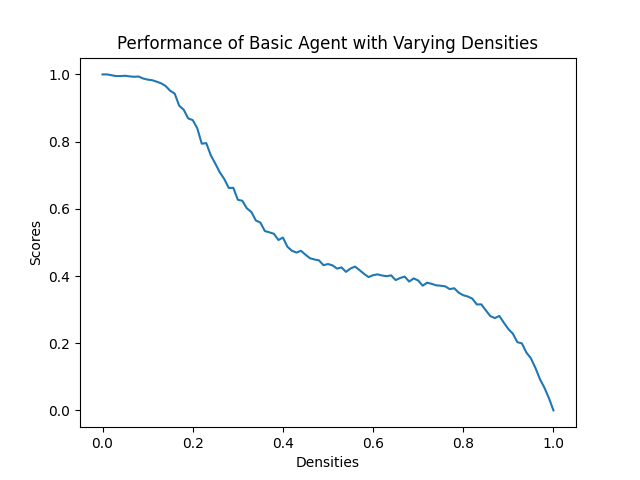
\includegraphics[width=\textwidth]{Density Performance Test - Basic Agent.png}
\caption{Compares scores of the basic agent given different densities}
\label{Density Performance Test - Basic Agent}
\end{figure}
Score is calculated by the number of bombs safely found divided by the total number of bombs. As expected, the score decreased as the density increased. Because more random queries will be made by the agent as the density increases, there will be more bombs triggered. Minesweeper according to the basic agent seems to be "hard" around 0.2 density because a decline in successes with no bombs triggered starts.

\subsection*{Efficiency}
There were no space or time constraints when implementing. However, we could have improved in time by not checking the neighbors of some cells when unnecessary such as when all the neighbors are already visible. We could have improved space by not storing as much info, but that would have affected time by a lot.

\section*{Improved Agent}
The improved agent, or Boxed \& S.W.E.P.T (mineSweeper Wins Every Predicament Triumphantly), aims to make more complex decisions that the basic agent can not make. While it still incorporates logic used in the basic agent, the improved agent groups cells together so multiple clues can be used to perform logic.

\subsection*{Representation}
The board is represented the same way as the basic agent, with all the same information still being stored. The improved agent represents even more information, however. This agent stores groups of cells that are affected by clues from neighboring cells. Each group contains the interconnected cells that affect each other so logic can later be applied to them.

\subsection*{Inference}
For this agent, we use cells that have been queried to group unqueried cells together based on clues that affect them. Each of these groups then uses multiple clues to determine where bombs are located. The most prevalent example of this would be if three cells in a row had the clues "1 2 1". The basic agent would not be able to determine where the bombs are, however, the improved agent recognizes how the cell with clue 1 is affected by the cell with clue 2 and can determine where the mine is. This process can be repeated with each group again and again until the board is completed to the best of the AI's ability (which is still, of course, affected by the luck of the board).\\
The program deduces everything it can from a given clue before continuing. We can be sure of this because it must use a clue to its fullest extent by comparing it to other cells and clues before making decisions. If a piece of information can't deduce everything it can, it isn't used until surrounding information allows it to make a full deduction.

\subsection*{Decisions}
In the beginning of a game, the decision of which cell to query is random. Once the information from that query is gained, the improved agent at first moves in a similar way to the basic agent. The improved agent moves differently, however, in that it looks at unqueried cells that are affected by clues and sees where bombs are likely to be and which cells can be queried. Once the location of bombs are determined, unqueried, but safe, cells can be explored and provide more information to the agent.\\
To further explain how the agent makes decisions, we can look at the "1 2 1" example again. For the sake of the example, these clues are in the first row of a 2x3 grid, and the second row will be referred to as a, b, c. Based on the first clue, the bomb can be in position a OR b. The second clue reveals that bombs can be positions a AND b, a AND c, or b AND c. And the last clue states that the bomb can be in b OR c. The logic used in the agent runs through the probabilities of where a bomb can be located and uses logic to determine what bomb locations break the rules the clues establish. This is applied to each group repeatedly to discover more and more of the board.\\
In terms of what cells it decides to query next, it is based on the order the groups, and their cells, are inserted into their data structures. While the first query is random, afterwards groups are pulled from the list and then cells from that list are queried based on the logic previously described.

\subsection*{Performance}
With the improved agent, larger boards can be solved and with a higher success rate than the the basic agent. Minesweeper becomes hard when the agent has to use two or more clues to come to a conclusion on where bombs are located. The logic behinds this becomes more complex since where the bombs can be placed increases, providing more and more, possible placements.\\
As described in previous sections, the improved agent can solve situations such as "1 2 1" when the basic agent would run out of moves. Since it is able to draw logic from multiple clues, it can find more locations of bombs, imrpoving upon the basic algorithm.

\subsection*{Efficiency}
By grouping the cells, the improved agent allows for better performance. If the probability of where a bomb is was calculated for N uncovered cells, there would be 2\^N possible combinations. The grouping allows the program to focus solely on cells that are immediately affected and calculate probabilities based on the logic given by clues, reducing the 2\^N combinations.

\end{document}